%!TEX root = ../report.tex

\chapter{Introduction}

In recent years, deep learning has significantly impacted research in the field of computer vision. Variations of Convolutional Neural Network architectures have shown state of the art performance in computer vision tasks such as image classification \cite{DBLP:journals/corr/HeZRS15}, object detection \cite{DBLP:journals/corr/RedmonDGF15}, action recognition \cite{DBLP:journals/corr/SimonyanZ14} and semantic segmentation \cite{DBLP:journals/corr/abs-1802-02611}. A considerable part of this success comes from the supervised learning paradigm through which the networks are trained with labeled samples.

State of the art deep learning techniques in semantic segmentation also make use of the supervised learning paradigm. Semantic segmentation is treated as a pixel-wise classification problem with the goal of assigning a class from a list of desired classes to every pixel in an image. The resultant image splits objects of interest into different regions thereby achieving the intended segmentation into meaningful regions.

	\begin{figure}
		\centering
		\begin{subfigure}{.4\textwidth}
			\centering
			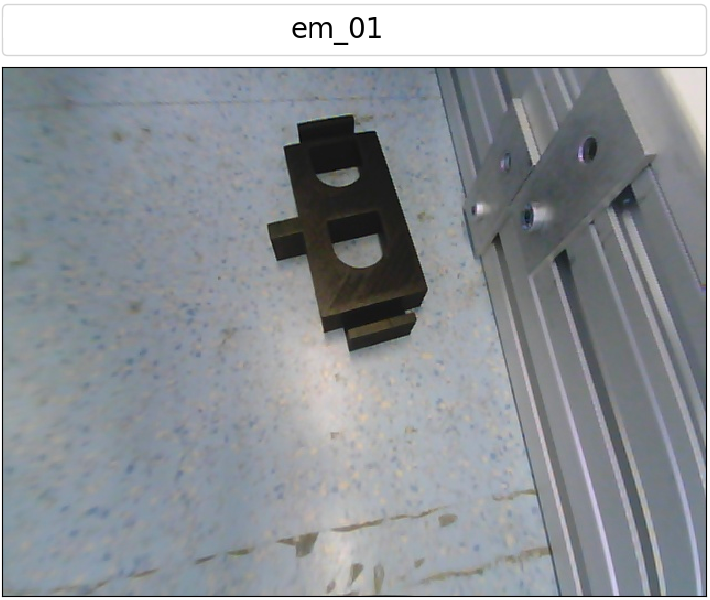
\includegraphics[width=1\linewidth]{images/classification}
			\caption{}
			\label{Fig:cls}
		\end{subfigure}
		\begin{subfigure}{.4\textwidth}
			\centering
			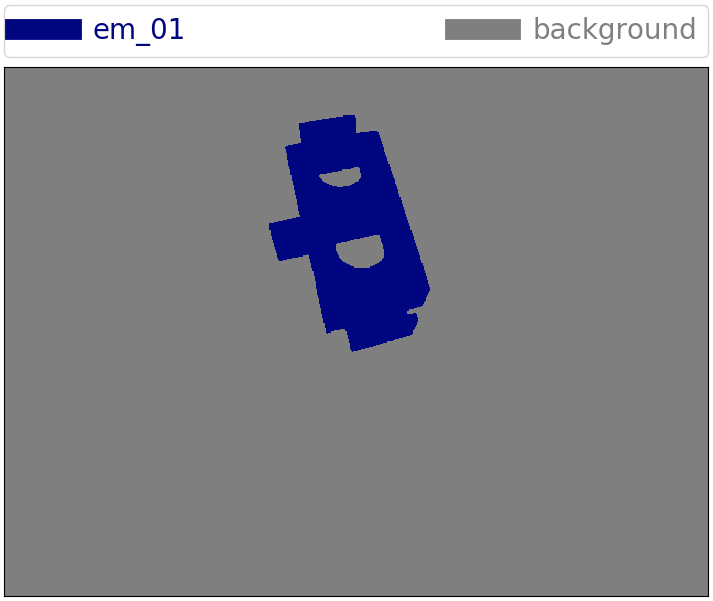
\includegraphics[width=1\linewidth]{images/segmentation}
			\caption{}
			\label{Fig:seg}
		\end{subfigure}
		\caption{(a) In image classification, we get the output "em\_01". (b) In semantic segmentation, we get an output image with each pixel labeled, from which we can infer that the image consists of "em\_01" and "background."}
		\label{Fig:clsseg}
	\end{figure}
	
Unlike the task of image classification (Figure \ref{Fig:cls}), where the location and boundaries of the desired object in an image are irrelevant, semantic segmentation (Figure \ref{Fig:seg}) requires the neural network to be able to spatially localize desired objects, delineate object boundaries and produce a single channel segmentation map (output image) which is of the same size as the input image.

\section{Motivation}

Semantic segmentation provides rich information from image space which could be interpreted to make useful inferences about the real world scene depicted by the image. We look at three potential applications of semantic segmentation which stand out to show the benefits of information obtained through semantic segmentation. 

\subsection{Potential applications}

Semantic segmentation can be used in autonomous cars to segment a road scene and extract information such as where the road is, where pedestrians are and so on. Figure \ref{Fig:appauto} shows an example of one such road scene segmentation. In robotics, an example application would be the segmentation of an indoor dining room shown in Figure \ref{Fig:approbo}. A robot could use this information to identify plates, chairs and so on. In augmented reality, an augmented dog could be placed on a sidewalk to walk a person to his destination as illustrated in Figure \ref{Fig:appaug}. 

	\begin{figure}
		\centering
		\begin{subfigure}{.3\textwidth}
			\centering
			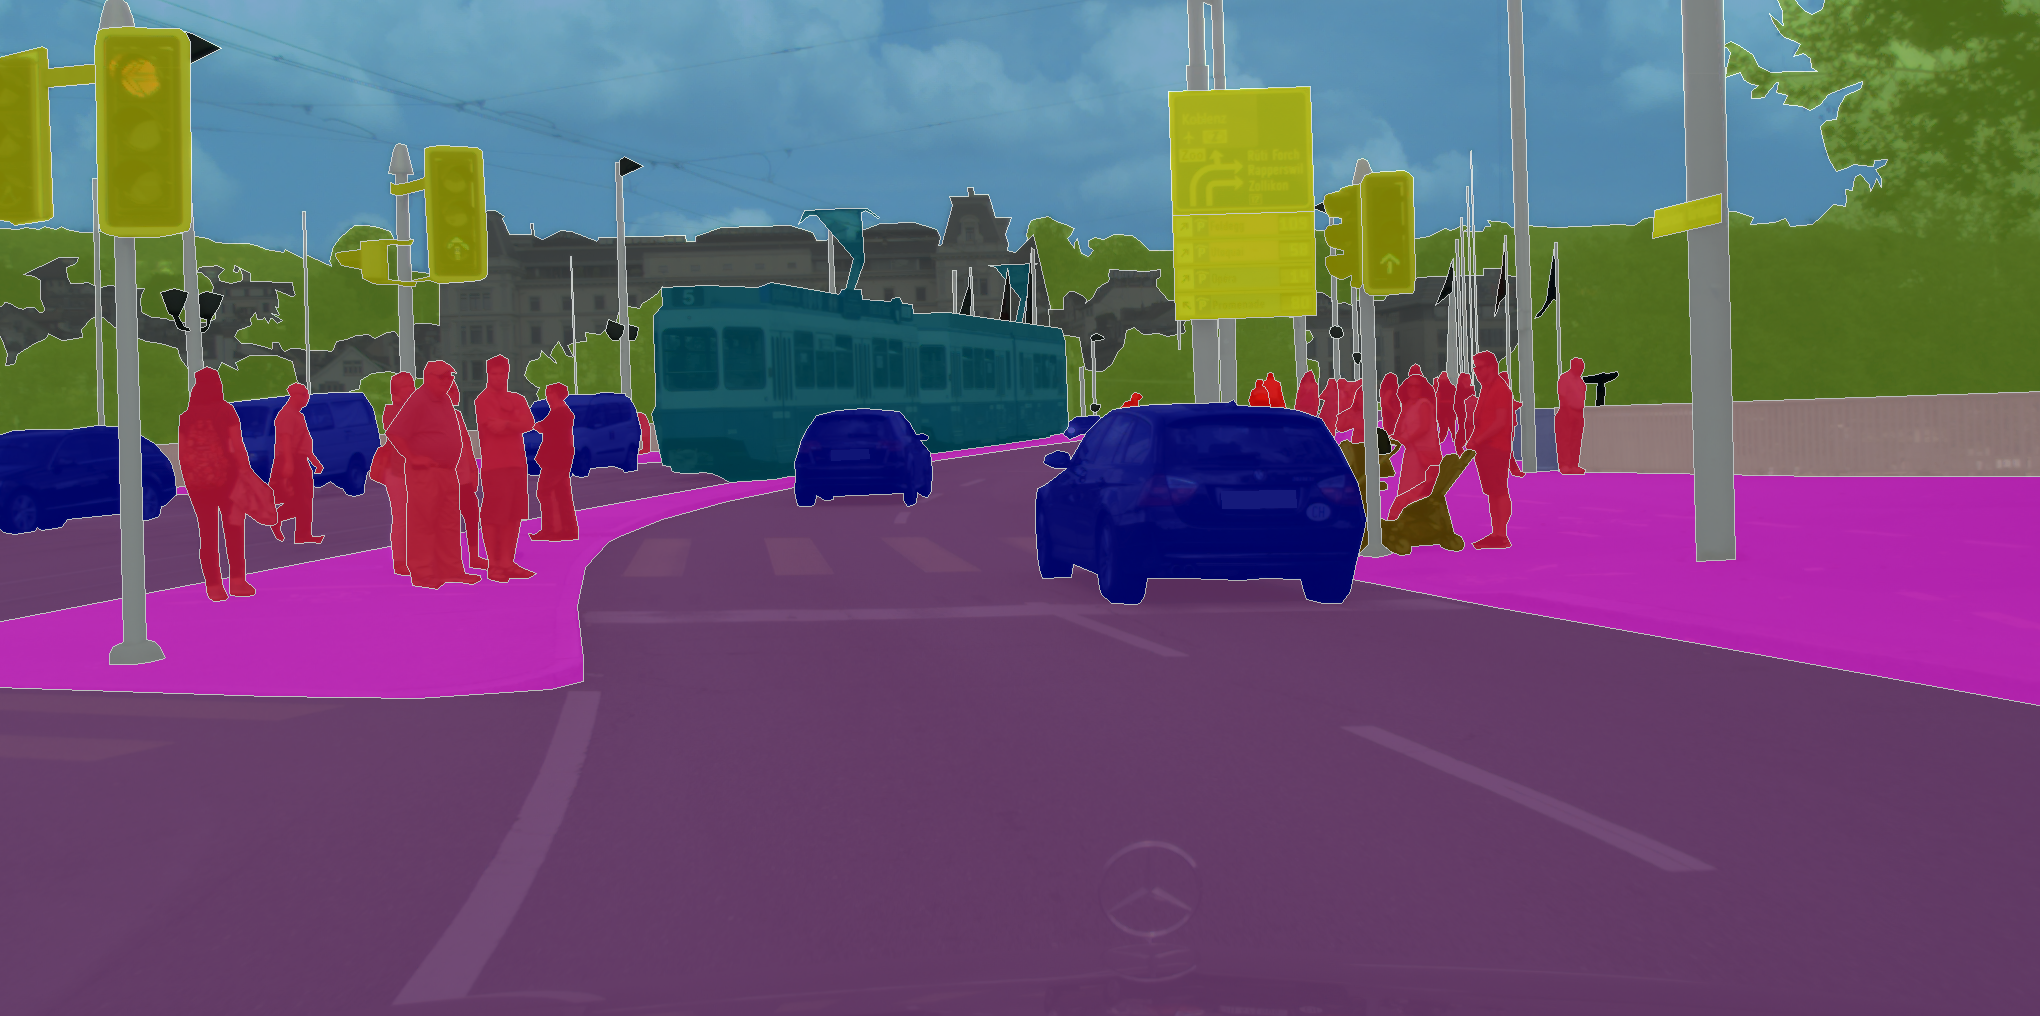
\includegraphics[width=.95\linewidth]{images/auto_driving}
			\caption{}
			\label{Fig:appauto}
		\end{subfigure}
		\begin{subfigure}{.3\textwidth}
			\centering
			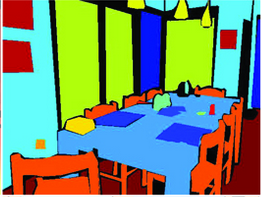
\includegraphics[width=.8\linewidth]{images/indoor}
			\caption{}
			\label{Fig:approbo}
		\end{subfigure}
		\begin{subfigure}{.3\textwidth}
			\centering
			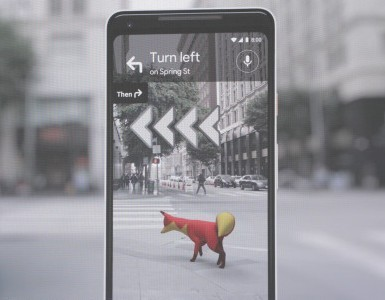
\includegraphics[width=.8\linewidth]{images/vr_dog}
			\caption{}
			\label{Fig:appaug}
		\end{subfigure}
		\caption{(a) Street scene \cite{cityscapes}, (b) Indoor environment \cite{indoor}, (c) Augmented guide \cite{techcrunch}.}
		\label{Fig:app}
	\end{figure}


\section{Challenges and Difficulties}

In this section, we look at the difficulties posed by the task of semantic segmentation in a deep learning setting.

\subsection{Labeling cost}

As semantic segmentation is a pixel-wise classification task, every pixel in the ground truth image needs to be labeled. This labeling can be achieved by first performing accurate object boundary delineation and later annotate each region with the corresponding class. Since objects could have a variety of shapes, this boundary delineation becomes difficult. Object occlusions and image space cluttered with objects further add to this difficulty.

\subsection{Context knowledge}

Different features could represent objects in general. In a local context, where only a small region inside an object is considered, different objects might have very similar features. Figures \ref{Fig:em01l} and \ref{Fig:motorl} illustrate the selection of two local regions within two different objects. By looking into just these selected regions, it is difficult to the classify the pixels within the regions as in a local context the two objects are similar. However, when a global context is gathered as illustrated in Figures \ref{Fig:em01g} and \ref{Fig:motorg}, the two objects become distinct, and it is now possible to classify the pixels within these regions. Therefore, for the task of semantic segmentation, gathering global context is important. 

	\begin{figure}[h]
		\centering
		\begin{subfigure}{.4\textwidth}
			\centering
			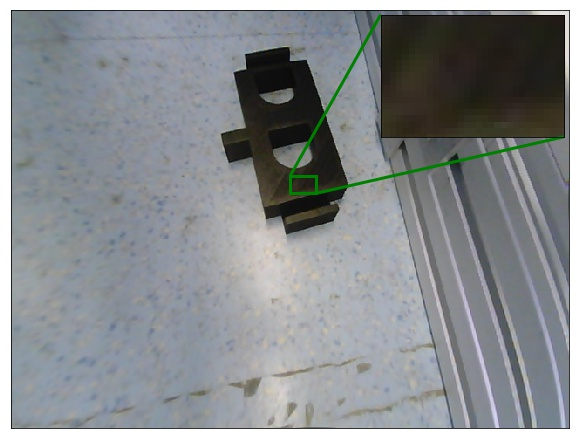
\includegraphics[width=.9\linewidth]{images/em_01_context_l}
			\caption{}
			\label{Fig:em01l}
		\end{subfigure}
		\begin{subfigure}{.4\textwidth}
			\centering
			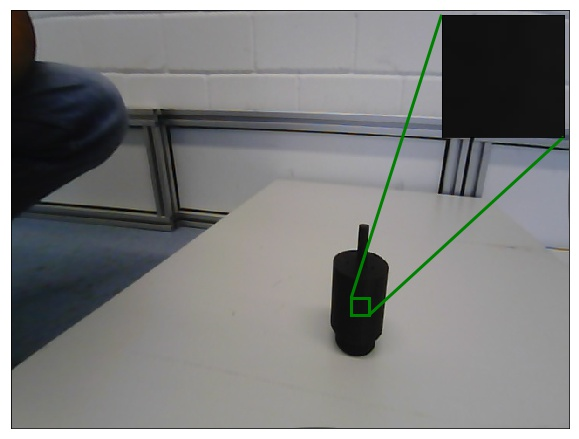
\includegraphics[width=.9\linewidth]{images/motor_context_l}
			\caption{}
			\label{Fig:motorl}
		\end{subfigure}
		\begin{subfigure}{.4\textwidth}
			\centering
			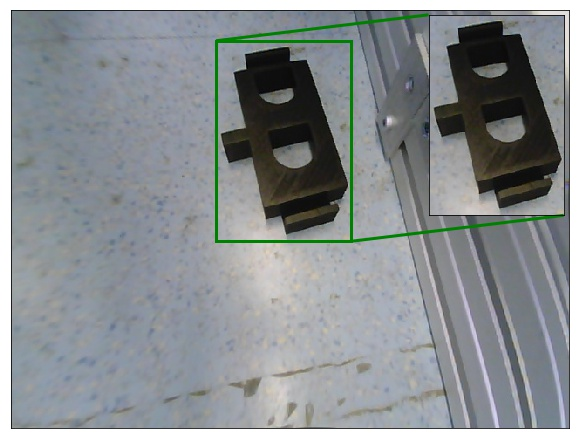
\includegraphics[width=.9\linewidth]{images/em_01_context_g}
			\caption{}
			\label{Fig:em01g}
		\end{subfigure}
		\begin{subfigure}{.4\textwidth}
			\centering
			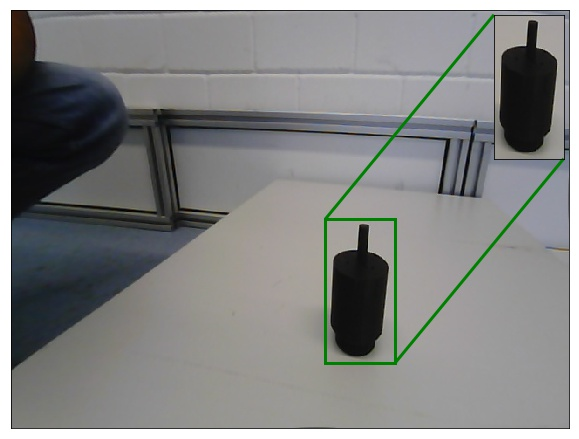
\includegraphics[width=.9\linewidth]{images/motor_context_g}
			\caption{}
			\label{Fig:motorg}
		\end{subfigure}
		\caption{Illustration of a local region in (a) "em\_01" and (b) "motor". The two local regions provide local context. Illustration of region containing an entire object shown in (c) "em\_01" and (d) "motor". The regions illustrated in (c) and (d) can be said to provide global context of corresponding objects.}
		\label{Fig:context}
	\end{figure}

\section{Problem Statement}

Existing benchmark datasets are not suitable when the objects needed to be segmented do not exist in them. Therefore, a semantic segmentation dataset needs to be created for the Robocup @Work objects. However, creating manual annotations for semantic segmentation is time-consuming because of the need to delineate boundaries of @Work objects which have a variety of shapes. Creating manual annotations is possible for only a limited number of images because of this time-consuming nature. Therefore, alternative methods need to be considered to improve the diversity and size of the dataset. One such alternative method is the creation of artificial images and using the existing manual labels to create annotations for these artificial images automatically. It is imperative that these artificial images add diversity to the dataset in terms of object scales, occlusions and so on. 

Besides, the semantic segmentation deep learning models selected are required to be resource efficient in terms of both memory and inference time. These models are also required to segment @Work objects with considerable accuracy.